\section{Introduction}
\label{sec:intro}

A 3D copy of a real room that looks real and can be explored on foot is useful for visiting a place remotely, for planning changes to a space and for testing robots that move indoors \cite{chen2026neverwhere, liu2026navgsim}. Neural radiance fields \cite{mildenhall2020nerf} and 3D Gaussian splatting (3DGS) \cite{kerbl3dgs} reconstruct such copies from photographs, and 3DGS renders them in real time. Capture has become cheap: an iPhone records each frame with its own camera pose from ARKit, and the Pro models add a LiDAR depth map.

Getting from a phone capture to a room one can walk in still has two weak points. First, rooms are dominated by plain walls, ceilings and floors. Camera poses estimated from the images fail on such surfaces, and the trained model has little to constrain its geometry; DN-Splatter \cite{turkulainen2025dnsplatter} and later methods \cite{ren2025agsmesh, ruan2025indoorgs, jin2025planargs} add depth, normal or planar priors for this reason. Second, walking needs collision that stops the walker at the walls. The SuperSplat Viewer's walk mode \cite{supersplatwalk, supersplatviewer} builds it automatically from the splat with splat-transform \cite{splattransform}, but we found no measurement of how closely this collision follows the real walls.

Our first attempt (v1, August--September 2026) estimated poses from images and failed on a plain-walled bedroom (Section~\ref{sec:journey}). We restarted as RoomRecon v2 around one rule: reuse maintained tools and write only the glue between them. The phone supplies poses and depth, DN-Splatter on nerfstudio \cite{tancik2023nerfstudio} trains the model on a shared GPU, and splat-transform and the SuperSplat Viewer provide collision and walking on a laptop (Figure~\ref{fig:teaser}).

\begin{figure}[!htb]
	\centering
	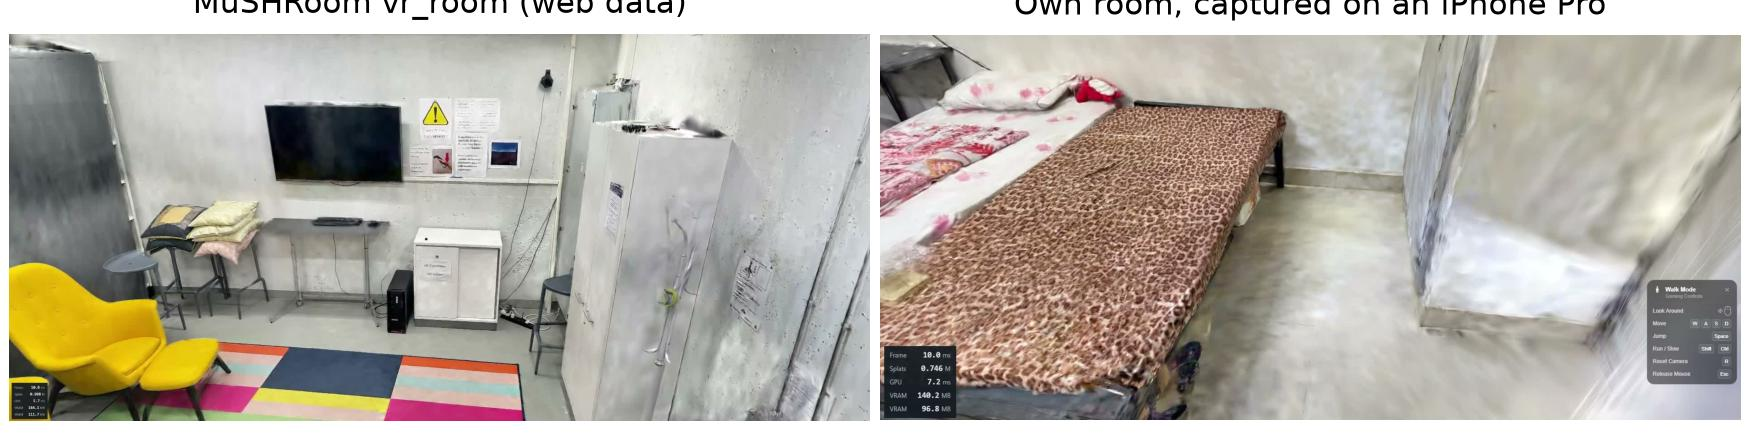
\includegraphics[width=\linewidth]{figures/teaser.jpg}
	\caption{First-person walk in the SuperSplat Viewer on a laptop (RTX~3050, 6\,GB), frames from our screen recordings. Left: MuSHRoom \texttt{vr\_room} (0.91\,M Gaussians). Right: our own room, captured on an iPhone~13~Pro (0.75\,M Gaussians). The lower-left overlay is the viewer's frame-time counter.}
	\label{fig:teaser}
\end{figure}

The salient contributions of this work are:
\begin{enumerate}
    \item \textbf{A working pipeline from an iPhone capture to a walkable Gaussian splat}, assembled from existing tools plus our glue (training settings for a shared GPU, automatic alignment of up direction, floor, scale and starting point, offline demo bundles), shown on a public room with a laser scan (MuSHRoom \texttt{vr\_room} \cite{ren2024mushroom}) and on our own room.
    \item \textbf{A measurement of walk-collision accuracy against a laser scan}, comparing collision built from DN-Splatter's mesh with the default built from the splat, with raw phone LiDAR and with Polycam's mesh, under criteria fixed before the run.
    \item \textbf{An account of what we explored and learned}, including the v1 failures that shaped v2 and two novelty attempts that failed their pre-agreed tests and are reported as negative results.
\end{enumerate}

The organisation of the report is as follows. Section~\ref{sec:related} discusses related work and its limitations. Section~\ref{sec:journey} describes how we explored the problem and what we learned. Section~\ref{sec:method} presents the pipeline and the collision evaluation. Section~\ref{sec:results} gives the datasets, setup and results, including a comparison with existing implementations. Section~\ref{sec:conclusion} concludes with two directions for future work.
